\documentclass[../DoAn.tex]{subfiles}
\begin{document}

Chương 2 đã trình bày về kiến trúc mạng Hyperledger Fabirc. Chương 3 này sẽ
tiến hành phần tích yêu cầu hệ thống triển khai mạng và ứng dụng phi tập trung
dựa trên nền tảng Hyperledger Fabric.
% Chương này có độ dài từ 9 đến 11 trang.

% Với phương pháp phân tích thiết kế hướng đối tượng, sinh viên sử dụng biểu đồ use case theo hướng dẫn của template này. Với các phương pháp khác, sinh viên trao đổi với giáo viên hướng dẫn để đổi tên và sắp xếp lại đề mục cho phù hợp. Ví dụ, thay vì sử dụng biểu đồ use case, sinh viên đi theo hướng tiếp cận Agile có thể dùng User Story.

% \section{Khảo sát hiện trạng}
% \label{section:2.1}
% Thông thường, khảo sát chi tiết về hiện trạng và yêu cầu của phần mềm sẽ được lấy từ ba nguồn chính, đó là (i) người dùng/khách hàng, (ii) các hệ thống đã có, (iii) và các ứng dụng tương tự.
% Sinh viên cần tiến hành phân tích, so sánh, đánh giá chi tiết ưu nhược điểm của các sản phẩm/nghiên cứu hiện có. Sinh viên có thể lập bảng so sánh nếu cần thiết. Kết hợp với khảo sát người dùng/khách hàng (nếu có), sinh viên nêu và mô tả sơ lược các tính năng phần mềm quan trọng cần phát triển.

\section{Tổng quan chức năng}
\label{section:2.2}

\subsection{Biểu đồ use case tổng quan}
\label{subsection:2.2.1}

\begin{figure}[h]
  \centering
  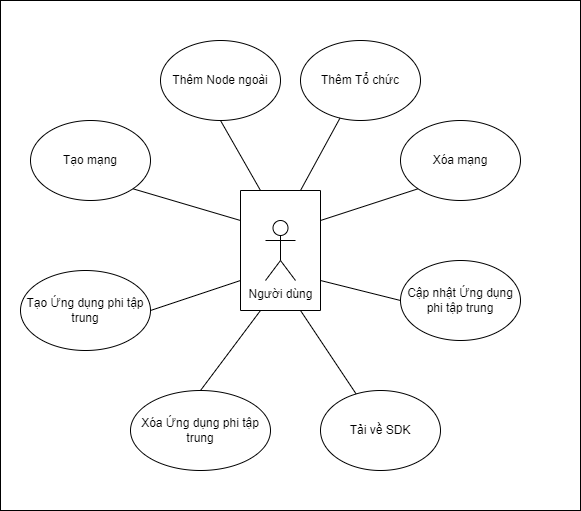
\includegraphics[width=0.75\linewidth]{Hinhve/DoAn-usecase.drawio.png}
  \caption[Biểu đồ usecase Tổng quan]{Biểu đồ usecase Tổng quan}
  \label{fig:general_usecase}
\end{figure}

Hình~\ref{fig:general_usecase} là biểu đồ usecase tổng quát của hệ thống. Hệ
thống chỉ bao gồm duy nhất một tác nhân, đó là người dùng. Người dùng có thể
tạo, xóa mạng Hyperledger Fabric. Đối với các mạng đã được tạo, người dùng có
thể thêm một node ngoài vào trong hệ thống, cùng với đó là thêm một tổ chức
mới. Trên các mạng đó, người dùng còn có thể tạo ứng dụng phi tập trung mới,
cập nhật và xóa các ứng dụng phi tập trung đã tồn tại. Cuối cùng, người dùng có
thể tải về các SDK để tương tác với các ứng dụng phi tập trung tương ứng.

% \subsection{Biểu đồ use case phân rã XYZ}
% \label{subsection:2.2.2}
% Với mỗi use case mức cao trong biểu đồ use case tổng quan, sinh viên tạo một mục riêng như mục \ref{subsection:2.2.2} và tiến hành phân rã use case đó. Lưu ý tên use case cần phân rã trong biểu đồ use case tổng quan phải khớp với tên đề mục.

% Trong mỗi mục như vậy, sinh viên vẽ và giải thích ngắn gọn các use case phân rã.

% \subsection{Quy trình nghiệp vụ}
% \label{subsection:2.2.2}
% Nếu sản phẩm/hệ thống cần xây dựng có quy trình nghiệp vụ quan trọng/đáng chú ý, sinh viên cần mô tả và vẽ biểu đồ hoạt động minh họa quy trình nghiệp vụ đó. Sinh viên lưu ý đây không phải là luồng sự kiện của từng use case, mà là luồng hoạt động kết hợp nhiều use case để thực hiện một nghiệp vụ nào đó.

% Ví dụ, một hệ thống quản lý thư viện có quy trình nghiệp vụ mượn trả với mô tả sơ bộ như sau: Sinh viên làm thẻ mượn, sau đó sinh viên đăng ký mượn sách, thủ thư cho mượn, và cuối cùng sinh viên trả lại sách cho thư viện. Một hệ thống có thể có một vài quy trình nghiệp vụ quan trọng như vậy.
\section{Đặc tả chức năng}
\label{section:2.3}

\newpage
\subsection{Đặc tả use case Tạo mạng}
\hfill

\begingroup
\renewcommand{\arraystretch}{1.5} % Default value: 1
\begin{table}[H]
  \centering
  \def\arraystretch{1.5}
  \caption{Đặc tả ca sử dụng “Tạo mạng”}
  \begin{tabular}{|p{0.2\textwidth}|p{0.75\textwidth}|}
    \hline
    Mã use case:          & UC01                                                                                                                                                                         \\ \hline
    Tên use case:         & Tạo mạng                                                                                                                                                                     \\ \hline
    Tác nhân:             & Người dùng                                                                                                                                                                   \\ \hline
    Mô tả:                & Người dùng tạo một mạng Hyperledger Fabric mới                                                                                                                               \\ \hline
    Điều kiện tiên quyết: & Người dùng đã đăng nhập vào hệ thống                                                                                                                                         \\ \hline
    Hậu điều kiện:        & Hiện thị kết quả tạo mạng                                                                                                                                                    \\ \hline
    Luồng sự kiện chính:  & \begin{tabular}{|p{0.05\textwidth}|p{0.15\textwidth}|p{0.465\textwidth}|}
                              STT & Thực hiện bởi & Hành động                                                                                                                                \\ \hline
                              1   & Người dùng    & Nhấn nút tạo mạng trên giao diện                                                                                                         \\ \hline
                              2   & Người dùng    & Nhập thông tin cấu hình mạng: (i) Tên mạng, (ii) Số máy ảo, (iii) Cấu hình mỗi máy ảo, (iv) Số Tổ chức, (v) Số peer node cho mỗi tổ chức \\ \hline
                              3   & Hệ thống      & Tự động triển khai mạng theo thông tin người dùng đã nhập                                                                                \\
                            \end{tabular} \\ \hline
    Luồng sự kiện con:    & Không có.                                                                                                                                                                    \\ \hline
    Ngoại lệ:             & Thông tin nhập vào không hợp lệ. Hệ thống sẽ thông báo lỗi.                                                                                                                  \\ \hline
    Bao gồm:              & Không có.                                                                                                                                                                    \\ \hline
  \end{tabular}
\end{table}
\endgroup

\newpage
\subsection{Đặc tả use case Thêm node ngoài}
\hfill

\begingroup
\renewcommand{\arraystretch}{1.5} % Default value: 1
\begin{table}[H]
  \centering
  \def\arraystretch{1.5}
  \caption{Đặc tả ca sử dụng “Thêm Node ngoài”}
  \begin{tabular}{|p{0.2\textwidth}|p{0.75\textwidth}|}
    \hline
    Mã use case:          & UC02                                                                                                                                                       \\ \hline
    Tên use case:         & Thêm Node ngoài                                                                                                                                            \\ \hline
    Tác nhân:             & Người dùng                                                                                                                                                 \\ \hline
    Mô tả:                & Người dùng thêm một node ngoài vào một mạng đang hoạt động của mình                                                                                        \\ \hline
    Điều kiện tiên quyết: & Người dùng đã tạo một mạng                                                                                                                                 \\ \hline
    Hậu điều kiện:        & Hiện thị kết quả thêm node ngoài                                                                                                                           \\ \hline
    Luồng sự kiện chính:  & \begin{tabular}{|p{0.05\textwidth}|p{0.15\textwidth}|p{0.465\textwidth}|}
                              STT & Thực hiện bởi & Hành động                                                                                                                  \\ \hline
                              1   & Người dùng    & Nhấn nút thêm node ngoài trên giao diện                                                                                    \\ \hline
                              2   & Người dùng    & Nhập thông tin: (i) Tên node, (ii) Tổ chức Node sẽ thuộc về, (iii) Địa chỉ IP và cổng mạng node sẽ hoạt động               \\ \hline
                              3   & Hệ thống      & Thực hiện sinh các tệp tin để có thể cho phép một Node ngoài với thông tin người dùng đã cung cấp có thể tham gia vào mạng \\ \hline
                              4   & Người dùng    & Tải tệp tin hệ thống sinh ra về                                                                                            \\ \hline
                              5   & Người dùng    & Khởi chạy các tệp tin được hệ thống sinh trên máy có đại chỉ Ip và cổng mạng lúc nhập để máy đó tham gia vào mạng          \\
                            \end{tabular} \\ \hline
    Luồng sự kiện con:    & Không có.                                                                                                                                                  \\ \hline
    Ngoại lệ:             & Thông tin nhập vào không hợp lệ, mạng chưa hoạt động. Hệ thống sẽ thông báo lỗi.                                                                           \\ \hline
    Bao gồm:              & Không có.                                                                                                                                                  \\ \hline
  \end{tabular}
\end{table}
\endgroup

\newpage
\subsection{Đặc tả use case Thêm tổ chức}
\hfill

\begingroup
\renewcommand{\arraystretch}{1.5} % Default value: 1
\begin{table}[H]
  \centering
  \def\arraystretch{1.5}
  \caption{Đặc tả ca sử dụng “Thêm tổ chức”}
  \begin{tabular}{|p{0.2\textwidth}|p{0.75\textwidth}|}
    \hline
    Mã use case:          & UC03                                                                                                             \\ \hline
    Tên use case:         & Thêm tổ chức                                                                                                     \\ \hline
    Tác nhân:             & Người dùng                                                                                                       \\ \hline
    Mô tả:                & Người dùng thêm một tổ chức mới vào một mạng đang hoạt động của mình                                             \\ \hline
    Điều kiện tiên quyết: & Người dùng đã tạo một mạng                                                                                       \\ \hline
    Hậu điều kiện:        & Hiện thị kết quả thêm tổ chức                                                                                    \\ \hline
    Luồng sự kiện chính:  & \begin{tabular}{|p{0.05\textwidth}|p{0.15\textwidth}|p{0.465\textwidth}|}
                              STT & Thực hiện bởi & Hành động                                                                   \\ \hline
                              1   & Người dùng    & Nhấn nút thêm tổ chức trên giao diện                                        \\ \hline
                              2   & Người dùng    & Nhập thông tin tổ chức mới: (i) Tên tổ chức, (ii) Số peer thuộc tổ chức mới \\ \hline
                              3   & Hệ thống      & Tự động thêm một tổ chức mới vào mạng                                       \\
                            \end{tabular} \\ \hline
    Luồng sự kiện con:    & Không có.                                                                                                        \\ \hline
    Ngoại lệ:             & Thông tin nhập vào không hợp lệ, mạng chưa hoạt động. Hệ thống sẽ thông báo lỗi.                                 \\ \hline
    Bao gồm:              & Không có.                                                                                                        \\ \hline
  \end{tabular}
\end{table}
\endgroup

\newpage
\subsection{Đặc tả use case Xóa mạng}
\hfill

\begingroup
\renewcommand{\arraystretch}{1.5} % Default value: 1
\begin{table}[H]
  \centering
  \def\arraystretch{1.5}
  \caption{Đặc tả ca sử dụng “Xóa mạng”}
  \begin{tabular}{|p{0.2\textwidth}|p{0.75\textwidth}|}
    \hline
    Mã use case:          & UC04                                                                         \\ \hline
    Tên use case:         & Xóa mạng                                                                     \\ \hline
    Tác nhân:             & Người dùng                                                                   \\ \hline
    Mô tả:                & Người dùng xóa một mạng của mình                                             \\ \hline
    Điều kiện tiên quyết: & Người dùng đã tạo một mạng                                                   \\ \hline
    Hậu điều kiện:        & Hiện thị kết quả xóa mạng                                                    \\ \hline
    Luồng sự kiện chính:  & \begin{tabular}{|p{0.05\textwidth}|p{0.15\textwidth}|p{0.465\textwidth}|}
                              STT & Thực hiện bởi & Hành động                               \\ \hline
                              1   & Người dùng    & Nhấn nút xóa mạng trên giao diện        \\ \hline
                              2   & Người dùng    & Xác nhận sẽ xóa mạng                    \\ \hline
                              3   & Hệ thống      & Gỡ bỏ toàn bỏ các thành phần trong mạng \\
                            \end{tabular} \\ \hline
    Luồng sự kiện con:    & Không có.                                                                    \\ \hline
    Ngoại lệ:             & Mạng chưa hoạt động. Hệ thống sẽ báo lỗi                                     \\ \hline
    Bao gồm:              & Không có.                                                                    \\ \hline
  \end{tabular}
\end{table}
\endgroup

\newpage
\subsection{Đặc tả use case Tạo Ứng dụng phi tập trung}
\hfill

\begingroup
\renewcommand{\arraystretch}{1.5} % Default value: 1
\begin{table}[H]
  \centering
  \def\arraystretch{1.5}
  \caption{Đặc tả ca sử dụng “Tạo Ứng dụng phi tập trung”}
  \begin{tabular}{|p{0.2\textwidth}|p{0.75\textwidth}|}
    \hline
    Mã use case:          & UC05                                                                                                                                                                                                          \\ \hline
    Tên use case:         & Tạo Ứng dụng phi tập trung                                                                                                                                                                                    \\ \hline
    Tác nhân:             & Người dùng                                                                                                                                                                                                    \\ \hline
    Mô tả:                & Người dùng tạo Ứng dụng phi tập trung trên một mạng đang hoạt động của mình                                                                                                                                   \\ \hline
    Điều kiện tiên quyết: & Người dùng đã tạo một mạng                                                                                                                                                                                    \\ \hline
    Hậu điều kiện:        & Hiện thị kết quả tạo ứng dụng phi tập trung                                                                                                                                                                   \\ \hline
    Luồng sự kiện chính:  & \begin{tabular}{|p{0.05\textwidth}|p{0.15\textwidth}|p{0.465\textwidth}|}
                              STT & Thực hiện bởi & Hành động                                                                                                                                                                \\ \hline
                              1   & Người dùng    & Nhấn nút tạo ứng dụng trên giao diện                                                                                                                                     \\ \hline
                              2   & Người dùng    & Nhập thông tin: (i) Tên ứng dụng, (ii) Mạng mà ứng dụng sẽ được triển khai lên, (iii) Kiểu mã hóa                                                                        \\ \hline
                              3   & Người dùng    & Thao tác trên giao diện để khai báo kiến trúc của ứng dụng: (i) Tạo thực thể, (ii) Thêm thuộc tính cho các thực thể, (iii) Thêm quan hệ cho các thực thể (1-1, 1-n, n-n) \\ \hline
                              4   & Người dùng    & Xác nhận tạo ứng dụng                                                                                                                                                    \\ \hline
                              5   & Hệ thống      & Tự động triển khai ứng dụng tương ứng lên mạng đã chọn                                                                                                                   \\ \hline
                              6   & Hệ thống      & Sinh ra SDK để có thể sử dụng ứng dụng.                                                                                                                                  \\
                            \end{tabular} \\ \hline
    Luồng sự kiện con:    & Không có.                                                                                                                                                                                                     \\ \hline
    Ngoại lệ:             & Thông tin nhập vào không hợp lệ, mạng chưa hoạt động. Hệ thống sẽ thông báo lỗi.                                                                                                                              \\ \hline
    Bao gồm:              & Không có.                                                                                                                                                                                                     \\ \hline
  \end{tabular}
\end{table}
\endgroup

\newpage
\subsection{Đặc tả use case Tải SDK}
\hfill

\begingroup
\renewcommand{\arraystretch}{1.5} % Default value: 1
\begin{table}[H]
  \centering
  \def\arraystretch{1.5}
  \caption{Đặc tả ca sử dụng “Tải SDK”}
  \begin{tabular}{|p{0.2\textwidth}|p{0.75\textwidth}|}
    \hline
    Mã use case:          & UC06                                                                     \\ \hline
    Tên use case:         & Tải SDK                                                                  \\ \hline
    Tác nhân:             & Người dùng                                                               \\ \hline
    Mô tả:                & Người dùng tải SDK tương ứng với một ứng dụng của mình                   \\ \hline
    Điều kiện tiên quyết: & Người dùng đã tạo một ứng dụng phi tập trung                             \\ \hline
    Hậu điều kiện:        & Hiện thị kết quả tải về SDK                                              \\ \hline
    Luồng sự kiện chính:  & \begin{tabular}{|p{0.05\textwidth}|p{0.15\textwidth}|p{0.465\textwidth}|}
                              STT & Thực hiện bởi & Hành động                       \\ \hline
                              1   & Người dùng    & Nhấn nút tải SDK trên giao diện \\ \hline
                              2   & Hệ thống      & Tải về tệp tin của SDK          \\ \hline
                              3   & Người dùng    & Sử dụng SDK                     \\ \hline
                            \end{tabular} \\ \hline
    Luồng sự kiện con:    & Không có.                                                                \\ \hline
    Ngoại lệ:             & Ứng dụng chưa hoạt động. Hệ thống sẽ thông báo lỗi.                      \\ \hline
    Bao gồm:              & Không có.                                                                \\ \hline
  \end{tabular}
\end{table}
\endgroup

\newpage
\subsection{Đặc tả use case Cập nhật Ứng dụng phi tập trung}
\hfill

\begingroup
\renewcommand{\arraystretch}{1.5} % Default value: 1
\begin{table}[H]
  \centering
  \def\arraystretch{1.5}
  \caption{Đặc tả ca sử dụng “Cập nhật Ứng dụng phi tập trung”}
  \begin{tabular}{|p{0.2\textwidth}|p{0.75\textwidth}|}
    \hline
    Mã use case:          & UC07                                                                                                                                                                                                                            \\ \hline
    Tên use case:         & Cập nhật Ứng dụng phi tập trung                                                                                                                                                                                                 \\ \hline
    Tác nhân:             & Người dùng                                                                                                                                                                                                                      \\ \hline
    Mô tả:                & Người dùng cập nhật một ứng dụng phi tập trung của mình                                                                                                                                                                         \\ \hline
    Điều kiện tiên quyết: & Người dùng đã tạo một ứng dụng phi tập trung                                                                                                                                                                                    \\ \hline
    Hậu điều kiện:        & Hiện thị kết quả cập nhật ứng dụng                                                                                                                                                                                              \\ \hline
    Luồng sự kiện chính:  & \begin{tabular}{|p{0.05\textwidth}|p{0.15\textwidth}|p{0.465\textwidth}|}
                              STT & Thực hiện bởi & Hành động                                                                                                                                                                                  \\ \hline
                              1   & Người dùng    & Nhấn nút cập nhật ứng dụng trên giao diện                                                                                                                                                  \\ \hline
                              2   & Người dùng    & Nhập thông tin mới: Tên mới cho ứng dụng                                                                                                                                                   \\ \hline
                              3   & Người dùng    & Thao tác trên giao diện để chỉnh sửa kiến trúc của ứng dụng: (i) Thêm thực thể, (ii) Thêm thuộc tính cho thực thể mới và cũ, (iii) Thêm quan hệ cho các thực thể mới và cũ (1-1, 1-n, n-n) \\ \hline
                              4   & Người dùng    & Xác nhận cập nhật ứng dụng                                                                                                                                                                 \\ \hline
                              5   & Hệ thống      & Tự động triển khai cập nhật ứng dụng                                                                                                                                                       \\ \hline
                              6   & Hệ thống      & Cập nhật SDK mới                                                                                                                                                                           \\
                            \end{tabular} \\ \hline
    Luồng sự kiện con:    & Không có.                                                                                                                                                                                                                       \\ \hline
    Ngoại lệ:             & Thông tin nhập vào không hợp lệ, mạng chưa hoạt động, ứng dụng chưa hoạt động. Hệ thống sẽ thông báo lỗi.                                                                                                                       \\ \hline
    Bao gồm:              & Không có.                                                                                                                                                                                                                       \\ \hline
  \end{tabular}
\end{table}
\endgroup

\newpage
\subsection{Đặc tả use case Xóa Ứng dụng phi tập trung}
\hfill
\begingroup
\renewcommand{\arraystretch}{1.5} % Default value: 1
\begin{table}[H]
  \centering
  \def\arraystretch{1.5}
  \caption{Đặc tả ca sử dụng “Xóa Ứng dụng phi tập trung”}
  \begin{tabular}{|p{0.2\textwidth}|p{0.75\textwidth}|}
    \hline
    Mã use case:          & UC08                                                                      \\ \hline
    Tên use case:         & Xóa Ứng dụng phi tập trung                                                \\ \hline
    Tác nhân:             & Người dùng                                                                \\ \hline
    Mô tả:                & Người dùng xóa một ứng dụng phi tập trung của mình                        \\ \hline
    Điều kiện tiên quyết: & Người dùng đã tạo một ứng dụng phi tập trung                              \\ \hline
    Hậu điều kiện:        & Hiện thị kết quả xóa ứng dụng                                             \\ \hline
    Luồng sự kiện chính:  & \begin{tabular}{|p{0.05\textwidth}|p{0.15\textwidth}|p{0.465\textwidth}|}
                              STT & Thực hiện bởi & Hành động                            \\ \hline
                              1   & Người dùng    & Nhấn nút xóa ứng dụng trên giao diện \\ \hline
                              2   & Người dùng    & Xác nhận xóa ứng dụng                \\ \hline
                              3   & Hệ thống      & Xóa ứng dụng khỏi mạng               \\ \hline
                            \end{tabular} \\ \hline
    Luồng sự kiện con:    & Không có.                                                                 \\ \hline
    Ngoại lệ:             & Mạng chưa hoạt động, ứng dụng chưa hoạt động. Hệ thống sẽ thông báo lỗi.  \\ \hline
    Bao gồm:              & Không có.                                                                 \\ \hline
  \end{tabular}
\end{table}
\endgroup

\section{Yêu cầu phi chức năng}
\label{section:2.4}
Để các mạng, ứng dụng phi tập trung có thể được ứng dụng trong nghiệp vụ doanh nghiệp, tính ổn định của hệ thống mạng sẽ cần được đảm bảo. Cụ thể đó là khả năng chịu lỗi, tính khả dụng cao và khả năng phục hồi.

Chương 3 đã trình bày phần tích yêu cầu hệ thống. Từ những phân tích này, chương 4 sẽ trình bày các công nghệ được sử dụng để hoàn thành những yêu cầu cần đạt được.
%%%%%%%%%%%%%%%%%%%%%%%%%%%%%%%%%%%

\end{document}
